% TikZ Editor Test File
% This file demonstrates the TikZ WYSIWYG editor capabilities

\documentclass{article}
\usepackage{tikz}
\usetikzlibrary{arrows,positioning,shapes}

\begin{document}

\section{Basic Shapes}

% Simple circle
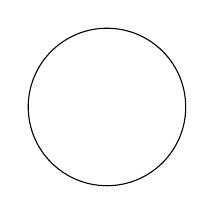
\begin{tikzpicture}
  \draw (0,0) circle (1);
\end{tikzpicture}

% Rectangle
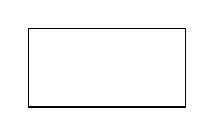
\begin{tikzpicture}
  \draw (0,0) rectangle (2,1);
\end{tikzpicture}

% Multiple shapes with colors
\begin{tikzpicture}
  \draw[red] (0,0) circle (1);
  \draw[blue,thick] (2,0) rectangle (4,1);
  \draw[green,dashed] (5,0) -- (7,1);
\end{tikzpicture}

\section{Nodes and Labels}

% Simple node

\begin{tikzpicture}
  \node at (0,0) {Hello};
\end{tikzpicture}

% Node with shape
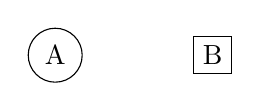
\begin{tikzpicture}
  \node[draw,circle] at (0,0) {A};
  \node[draw,rectangle] at (2,0) {B};
\end{tikzpicture}

\section{Complex Diagram}

% Flow chart example
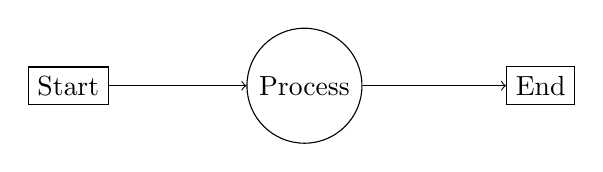
\begin{tikzpicture}
  \node[draw,rectangle] (start) at (0,0) {Start};
  \node[draw,circle] (process) at (3,0) {Process};
  \node[draw,rectangle] (end) at (6,0) {End};
  
  \draw[->] (start) -- (process);
  \draw[->] (process) -- (end);
\end{tikzpicture}

\section{Styled Elements}

% Various styles
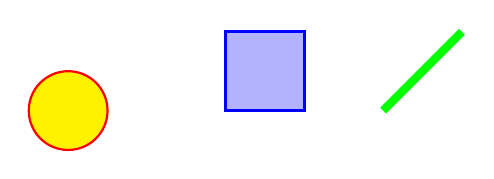
\begin{tikzpicture}
  \draw[fill=yellow,draw=red,thick] (0,0) circle (0.5);
  \draw[fill=blue!30,draw=blue,very thick] (2,0) rectangle (3,1);
  \draw[draw=green,line width=3pt] (4,0) -- (5,1);
\end{tikzpicture}

\section{Positioned Nodes}

% Grid of nodes
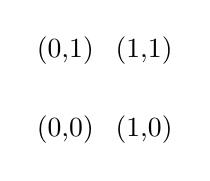
\begin{tikzpicture}
  \node at (0,0) {(0,0)};
  \node at (1,0) {(1,0)};
  \node at (0,1) {(0,1)};
  \node at (1,1) {(1,1)};
\end{tikzpicture}

\section{Click the "Edit TikZ" button above any diagram to open the visual editor!}

% Test diagram for editing
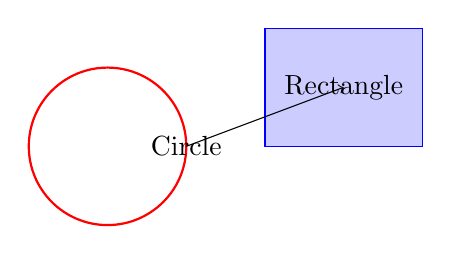
\begin{tikzpicture}
  \draw[red,thick] (0,0) circle (1);
  \draw[blue,fill=blue!20] (2,0) rectangle (4,1.5);
  \node at (1,0) {Circle};
  \node at (3,0.75) {Rectangle};
  \draw[->] (1,0) -- (3,0.75);
\end{tikzpicture}

\end{document}
